\documentclass[a4paper, 12pt]{article}
\usepackage[a4paper,top=1.5cm, bottom=1.5cm, left=1cm, right=1cm]{geometry}
\usepackage{cmap}					% поиск в PDF
\usepackage{mathtext} 				% русские буквы в формулах
\usepackage[T2A]{fontenc}			% кодировка
\usepackage[utf8]{inputenc}			% кодировка исходного текста
\usepackage[english,russian]{babel}	% локализация и переносы

\usepackage{amsmath}
\usepackage{indentfirst}
\usepackage{longtable}
\usepackage{graphicx}
\usepackage{array}
\usepackage{tikz}

\usepackage{wrapfig}
\usepackage{siunitx} % Required for alignment
\usepackage{subfigure}
\usepackage{multirow}
\usepackage{rotating}
\usepackage{caption}

\begin{document}
    

\thispagestyle{empty}

\begin{center}
\large{«Московский физико-технический институт»} \\  
\large{Физтех-школа радитехники и компьютерных технологий }\\
\vspace*{8cm}
{\bfseries
    {\Huge Перевод статьи <<O(1) алгоритм для реализации схемы вытеснения кэша LFU>>}
}
\end{center}

\vspace*{1cm}
\begin{flushright}

    \textbf{Авторы:} \\ Профессор Кетан Шах \\ Анирбан Митра \\ Дхрув Матани \\ 
    \hspace*{1cm} \\
    \textbf{Перевод:} \\Насыров Альмир

\end{flushright}

\vspace*{9cm}
\begin{center}
\small{г. Долгопрудный\\2024}
\end{center}

\newpage

\begin{abstract}
    Алгоритмы вытеснения кэша широко используются в операционных системах, базах данных и других системах, использующих кэши для ускорения выполнения за счет кэширования данных, которые используются приложением. Существуют различные алгоритмы, такие как MRU (Most Recently Used — наиболее недавно использованные), MFU (Most Frequently Used — наиболее часто использованные), LRU (Least Recently Used — наименее недавно использованные) и LFU (Least Frequently Used — наименее часто использованные), каждая из которых имеет свои преимущества и недостатки и, следовательно, используется в определенных сценариях. На сегодняшний день наиболее широко используемый алгоритм — это LRU, как из-за его скорости работы $O(1)$, так и из-за его сходства с поведением, ожидаемым от большинства приложений. Алгоритм LFU также имеет поведение, желательное для многих реальных рабочих нагрузок. Однако во многих случаях алгоритм LRU предпочитают алгоритму LFU из-за его меньшей сложности выполнения $O(1)$ против $O(\log{n})$. Здесь мы представляем алгоритм вытеснения кэша LFU, который имеет сложность выполнения O(1) для всех своих операций, включая вставку, доступ и удаление (вытеснение).
\end{abstract}

\section{Введение}

Статья организована следующим образом:

\begin{itemize}
    \item Описание случаев использования LFU, где он может оказаться превосходным по сравнению с другими алгоритмами вытеснения кэш
    \item Операции со словарем, которые должны поддерживаться реализацией кэша LFU. Это операции, которые определяют сложность выполнения стратегии
    \item Описание наилучшего известного в настоящее время алгоритма LFU вместе с его сложностью выполнения
    \item Описание предлагаемого алгоритма LFU, каждая операция которого имеет сложность выполнения $O(1)$
\end{itemize}

\section{Применение LFU}

Рассмотрим приложение прокси-сервера кэша для протокола HTTP. Этот прокси обычно располагается между интернетом и пользователем или набором пользователей. Он обеспечивает доступ всех пользователей к интернету и позволяет совместно использовать все общие ресурсы для оптимизации сетевого использования и улучшения отклика. Такой прокси-кэш должен стремиться к максимальному количеству данных, которые он может кэшировать в ограниченном объеме доступного хранилища или памяти.

Обычно многие статические ресурсы, такие как изображения, CSS-стили и JavaScript-код, могут быть легко закэшированы на довольно долгое время, прежде чем они будут заменены новыми версиями. Эти статические ресурсы или "ассеты", как их называют программисты, включены практически в каждую страницу, поэтому наиболее полезно кэшировать их, поскольку практически каждый запрос будет требовать их. Более того, поскольку прокси-сервер должен обслуживать тысячи запросов в секунду, накладные расходы на это должны быть минимальными.

Таким образом, прокси должен вытеснять только те ресурсы, которые не используются очень часто. Следовательно, часто используемые ресурсы должны сохраняться за счет менее часто используемых, поскольку первые доказали свою полезность с течением времени. Конечно, существует контраргумент, утверждающий, что ресурсы, которые ранее использовались активно, могут не потребоваться в будущем, но в большинстве случаев это не так. Например, статические ресурсы часто используемых страниц всегда запрашиваются каждым пользователем этой страницы. Следовательно, стратегия замены кэша LFU может быть использована такими прокси-серверами для вытеснения наименее часто используемых элементов из кэша, когда не хватает памяти.

LRU также может быть применимой стратегией здесь, но она будет неэффективна, когда шаблон запросов таков, что все запрашиваемые элементы не помещаются в кэш, и элементы запрашиваются циклически. В случае LRU элементы будут постоянно входить и выходить из кэша, и ни один пользовательский запрос не будет попадать в кэш. Однако в тех же условиях алгоритм LFU будет работать намного лучше, при этом большинство закэшированных элементов приведет к попаданию в кэш.

\section{Операции со словарем, поддерживаемые кэшем LFU}

Когда мы говорим об алгоритме вытеснения кэша, нам нужно учитывать три различных операции с кэшированными данными:

\begin{itemize}
    \item Установить (или вставить) элемент в кэш
    \item Извлечь (или найти) элемент в кэше, одновременно увеличив его счетчик использования (для LFU)
    \item Вытеснить (или удалить) наименее часто используемый элемент из кэша (или элемент, соответствующий стратегии вытеснения)
\end{itemize}

\section{Текущая наилучшая сложность алгоритма LFU}

На момент написания статьи лучшие известные времена выполнения для каждой из вышеупомянутых операций для стратегии вытеснения кэша LFU следующие:


\begin{itemize}
    \item Вставка: $O(\log{n})$
    \item Поиск: $O(\log{n})$
    \item Удаление: $O(\log{n})$
\end{itemize}

Эти значения сложности напрямую следуют из сложности реализации биномиальной кучи и стандартной таблицы хеширования без коллизий. Стратегия кэширования LFU может быть легко и эффективно реализована с использованием структуры данных min-куча и хеш-таблицы. Min-куча создается на основе счетчика использования (элемента), а хеш-таблица индексируется по ключу элемента. Все операции на хеш-таблице без коллизий имеют порядок O(1), поэтому время выполнения кэша LFU определяется временем выполнения операций на min-куче.

Когда элемент вставляется в кэш, он получает счетчик использования, равный 1, и поскольку вставка в min-кучу стоит $O(\log{n})$, вставка в кэш LFU занимает время $O(\log{n})$.

Когда элемент ищется, он находится с помощью функции хеширования, которая хеширует ключ в реальный элемент. Одновременно счетчик использования (счетчик в max-куче) увеличивается на один, что приводит к реорганизации min-кучи, и элемент перемещается от корня. Поскольку элемент может перемещаться вниз до log n уровней на любом этапе, эта операция также занимает время $O(\log{n})$.

Когда элемент выбирается для вытеснения и затем удаляется из кучи, это может вызвать значительную реорганизацию структуры данных кучи. Элемент с наименьшим счетчиком использования находится в корне min-кучи. Удаление корня min-кучи включает в себя замену корневого узла на последний листовой узел в куче и спуск этого узла до его правильного положения. Эта операция также имеет сложность выполнения $O(\log{n})$.

\section{Предлагаемый алгоритм LFU}

Предлагаемый алгоритм LFU имеет сложность выполнения $O(1)$ для каждой операции со словарем (вставка, поиск и удаление), которые могут выполняться на кэше LFU. Это достигается за счет поддержания двух связанных списков: одного по частоте доступа и одного для всех элементов, имеющих одинаковую частоту доступа.

Хеш-таблица используется для доступа к элементам по ключу (не показана на диаграмме для ясности). Двусвязный список используется для связывания узлов, представляющих набор узлов с одинаковой частотой доступа (показаны прямоугольными блоками на диаграмме ниже). Мы называем этот двусвязный список частотным списком. Этот набор узлов, имеющих одинаковую частоту доступа, фактически является двусвязным списком таких узлов (показаны круглыми узлами на диаграмме ниже). Мы называем этот двусвязный список (который является локальным для определенной частоты) списком узлов. Каждый узел в списке узлов имеет указатель на свой родительский узел в частотном списке (не показан на диаграмме для ясности). Таким образом, узлы x и y будут иметь указатель на узел 1, узлы z и a будут иметь указатель на узел 2 и так далее.

\begin{figure}[ht!]
    \begin{center}
        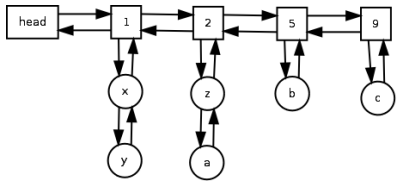
\includegraphics{6elem.png}
    \end{center}
    \caption{Словарь LFU с 6 элементами}
\end{figure}

\begin{figure}[ht!]
    \begin{center}
        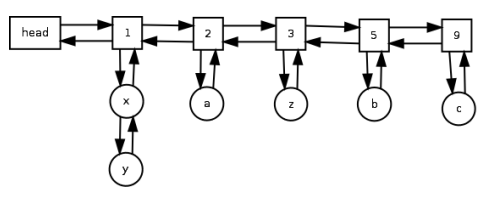
\includegraphics{after_k.png}
    \end{center}
    \caption{После того, как элемент с ключом 'z' был доступен вновь}
\end{figure}

Псевдокод ниже показывает, как инициализировать кэш LFU. Хеш-таблица, используемая для поиска элементов по ключу, обозначена переменной bykey. Мы используем множество (SET) вместо связанного списка для хранения элементов с одинаковой частотой доступа для простоты реализации. Переменная items — это стандартная структура данных SET, которая хранит ключи таких элементов, имеющих одинаковую частоту доступа. Ее вставка, поиск и удаление имеют сложность выполнения $O(1)$.

\newpage

\subsection*{Создание нового узла частоты}

\begin{verbatim}
NEW-FREQ-NODE()
01 Object o
02 o.value ← 0
03 o.items ← SET()
04 o.prev ← o
05 o.next ← o
06 return o
\end{verbatim}

\subsection*{Создание нового элемента LFU}

\begin{verbatim}
NEW-LFU-ITEM(data, parent)
01 Object o
02 o.data ← data
03 o.parent ← parent
04 return o
\end{verbatim}

\subsection*{Создание нового кэша LFU}

\begin{verbatim}
NEW-LFU-CACHE()
01 Object o
02 o.bykey ← HASH-MAP()
03 o.freq head ← NEW-FREQ-NODE()
04 return o
\end{verbatim}

Объект кэша LFU доступен через переменную \texttt{lfu cache}:
\begin{verbatim}
lfu cache ← NEW-LFU-CACHE()
\end{verbatim}

Мы также определяем несколько вспомогательных функций, которые помогают в манипуляции связанным списком.

\textit{Создаем новый узел и устанавливаем его указатели на предыдущий и следующий узлы}:
\begin{verbatim}
GET-NEW-NODE(value, prev, next)
01 nn ← NEW-FREQ-NODE()
02 nn.value ← value
03 nn.prev ← prev
04 nn.next ← next
05 prev.next ← nn
06 next.prev ← nn
07 return nn
\end{verbatim}

\textit{Удаляем (разрываем связь) узел из связанного списка:}
\begin{verbatim}
DELETE-NODE(node)
01 node.prev.next ← node.next
02 node.next.prev ← node.prev
\end{verbatim}

Изначально кэш LFU начинается как пустая хеш-таблица и пустой список частот. Когда первый элемент добавляется, создается единственный элемент в хеш-таблице, который указывает на этот новый элемент (по его ключу), и новый узел частоты со значением 1 добавляется в список частот. Очевидно, что количество элементов в хеш-таблице будет равно количеству элементов в кэше LFU. Новый узел добавляется в список частоты 1. Этот узел фактически указывает обратно на узел частоты, членом которого он является. Например, если узел \texttt{x} был добавлен, то узел \texttt{x} будет указывать обратно на узел частоты 1. Следовательно, сложность выполнения вставки элемента составляет $O(1)$. \\

\textit{Доступ (поиск) элемента в кэше LFU с одновременным увеличением его счетчика использования:}
\begin{verbatim}
ACCESS(key)
01 tmp ← lfu cache.bykey[key]
02 if tmp equals null then
03 throw Exception("No such key")
04 freq ← tmp.parent
05 next freq ← freq.next
06 if next freq equals lfu cache.freq head or
07 next freq.value does not equal freq.value + 1 then
08 next freq ← GET-NEW-NODE(freq.value + 1, freq, next freq)
09 next freq.items.add(key)
10 tmp.parent ← next freq
11 freq.items.remove(key)
12 if freq.items.length equals 0 then
13 DELETE-NODE(freq)
14 return tmp.data
\end{verbatim}

Когда этот элемент снова доступен, выполняется поиск узла частоты элемента и запрашивается значение его следующего узла. Если следующий узел не существует или значение следующего узла не на 1 больше текущего значения, то создается новый узел частоты со значением на 1 больше текущего значения узла частоты и вставляется в правильное место. Узел удаляется из текущего набора и вставляется в новый набор списка частот. Указатель частоты узла обновляется для указания на его новый узел частоты. Например, если узел \texttt{z} снова доступен, то он удаляется из списка частот со значением 2 и добавляется в список частот со значением 3. Следовательно, сложность выполнения доступа к элементу составляет O(1).\\

\textit{Вставка нового элемента в кэш LFU:}
\begin{verbatim}
INSERT(key, value)
01 if key in lfu cache.bykey then
02 throw Exception("Key already exists")
03 freq ← lfu cache.freq head.next
04 if freq.value does not equal 1 then
05 freq ← GET-NEW-NODE(1, lfu cache.freq head, freq)
06 freq.items.add(key)
07 lfu cache.bykey[key] ← NEW-LFU-ITEM(value, freq)
\end{verbatim}

Когда элемент с наименьшей частотой доступа нужно удалить, любой элемент из первого (крайнего левого) списка частот выбирается и удаляется. Если список узлов этой частоты становится пустым из-за этого удаления, то узел частоты также удаляется. Ссылка на элемент из хеш-таблицы также удаляется. Следовательно, сложность выполнения удаления наименее часто используемого элемента составляет O(1). \\ 

\textit{Получение элемента с наименьшей частотой использования (наименее часто используемого элемента) в кэше:}
\begin{verbatim}
GET-LFU-ITEM()
01 if lfu cache.bykey.length equals 0 then
02 throw Exception("The set is empty")
03 return lfu cache.bykey[lfu cache.freq head.next.items[0]]
\end{verbatim}

Таким образом, мы видим, что сложность выполнения каждой из операций со словарем в кэше LFU составляет O(1).




\end{document}